The panel below replaces the current panel~D (``Beyond \texttt{filter\_vep}'',
chromosome~22, segmental duplications) of the cache-workflow version of
Figure~1. It is generated by \nolinkurl{paper/figure1/build_tiered_annotation.py}
in the same draw.io/SVG style as the other panels and reads its numbers from
\texttt{results/}. The chromosome~22 segmental-duplication example can stay
in the supplement as the bedtools-verified equivalence check.

\begin{figure}[ht]
\centering
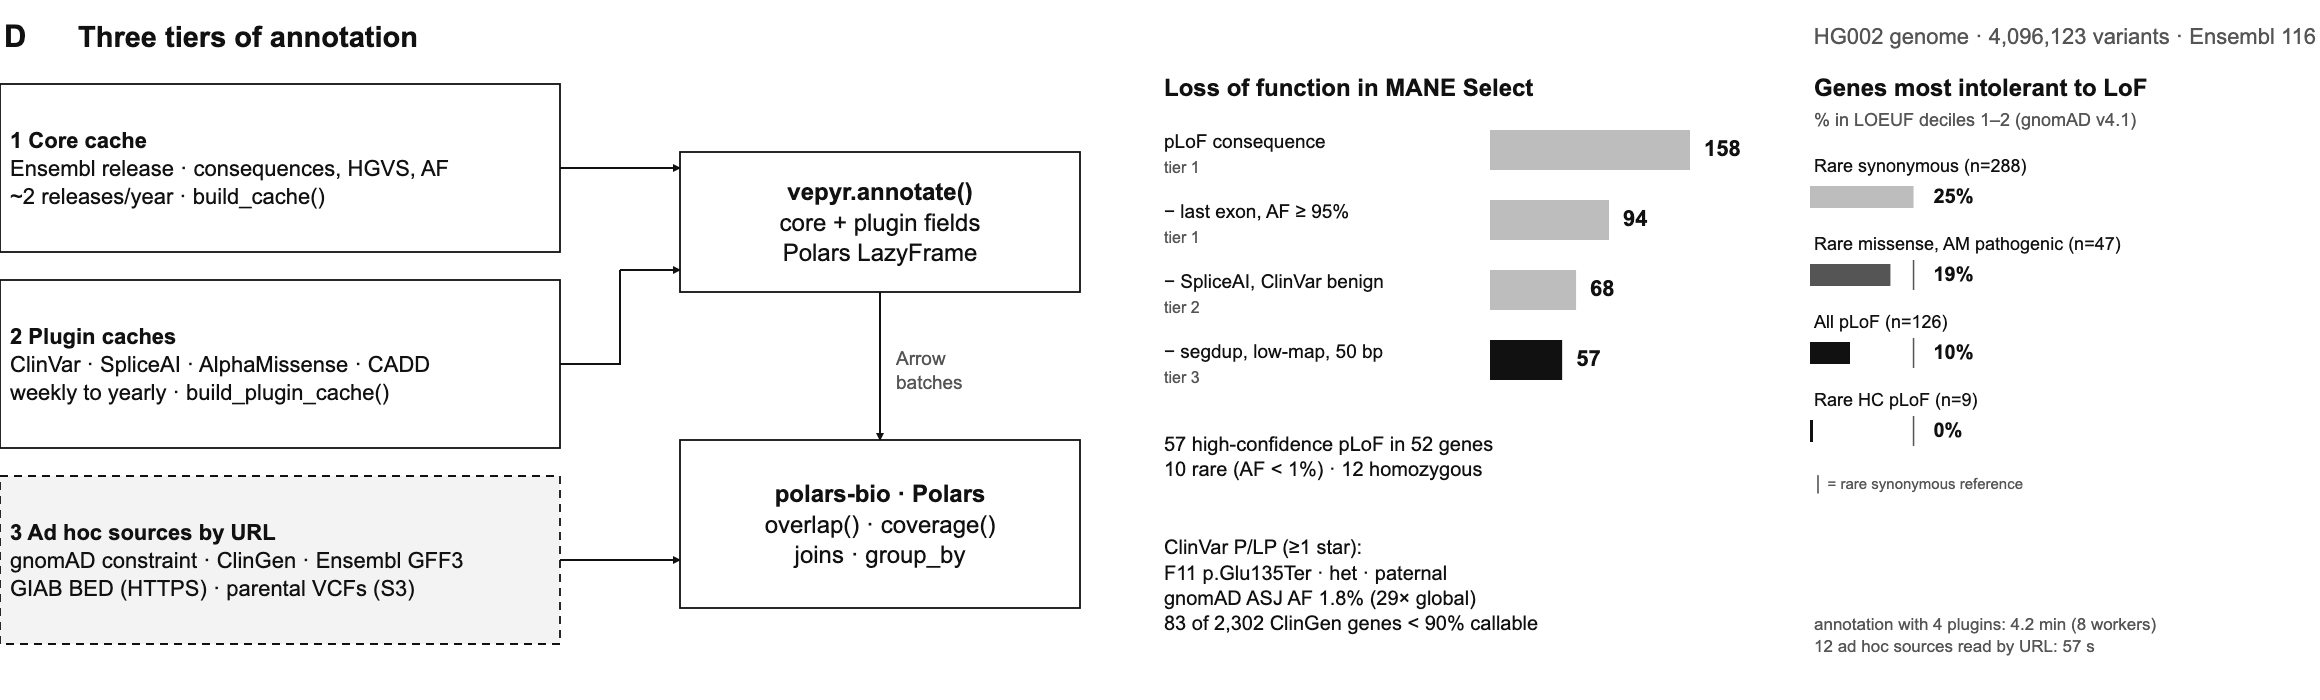
\includegraphics[width=\textwidth]{../figure1/d-tiered-annotation-proposal.png}
\caption*{\textbf{Figure 1D (proposal). Three tiers of annotation in the HG002
genome.} Core (tier~1) and plugin (tier~2) annotations are produced by
\texttt{vepyr.annotate()} from prebuilt Parquet caches that are refreshed at
different rates; ad hoc sources (tier~3) are read directly from their URLs by
polars-bio and Polars when the query runs and are combined with the annotated
frame by joins and interval operations (\texttt{overlap()},
\texttt{coverage()}). Middle: variants with a predicted loss-of-function
(pLoF) consequence in a MANE Select transcript that remain after the filters
contributed by each tier (last exon; SpliceAI support and ClinVar benign
classification; segmental duplications, low mappability and the 50-bp rule),
leaving \NHc{} high-confidence pLoF variants in \NHcGenes{} genes. Right:
share of each variant class in the 20\% of genes most intolerant to LoF
(gnomAD v4.1 LOEUF deciles 1--2); ticks mark the share of rare synonymous
variants. pLoF variants are depleted from these genes, as expected under
purifying selection. Bottom of the middle column: the only ClinVar
pathogenic variant with review criteria, the Ashkenazi founder allele
\textit{F11} \PlpHgvsp{}, with its parental origin from the parental VCFs,
and the number of ClinGen genes with less than 90\% of their coding sequence
in the benchmark regions. Details in Supplementary Section~X.}
\end{figure}

\begin{figure}[p]
\centering
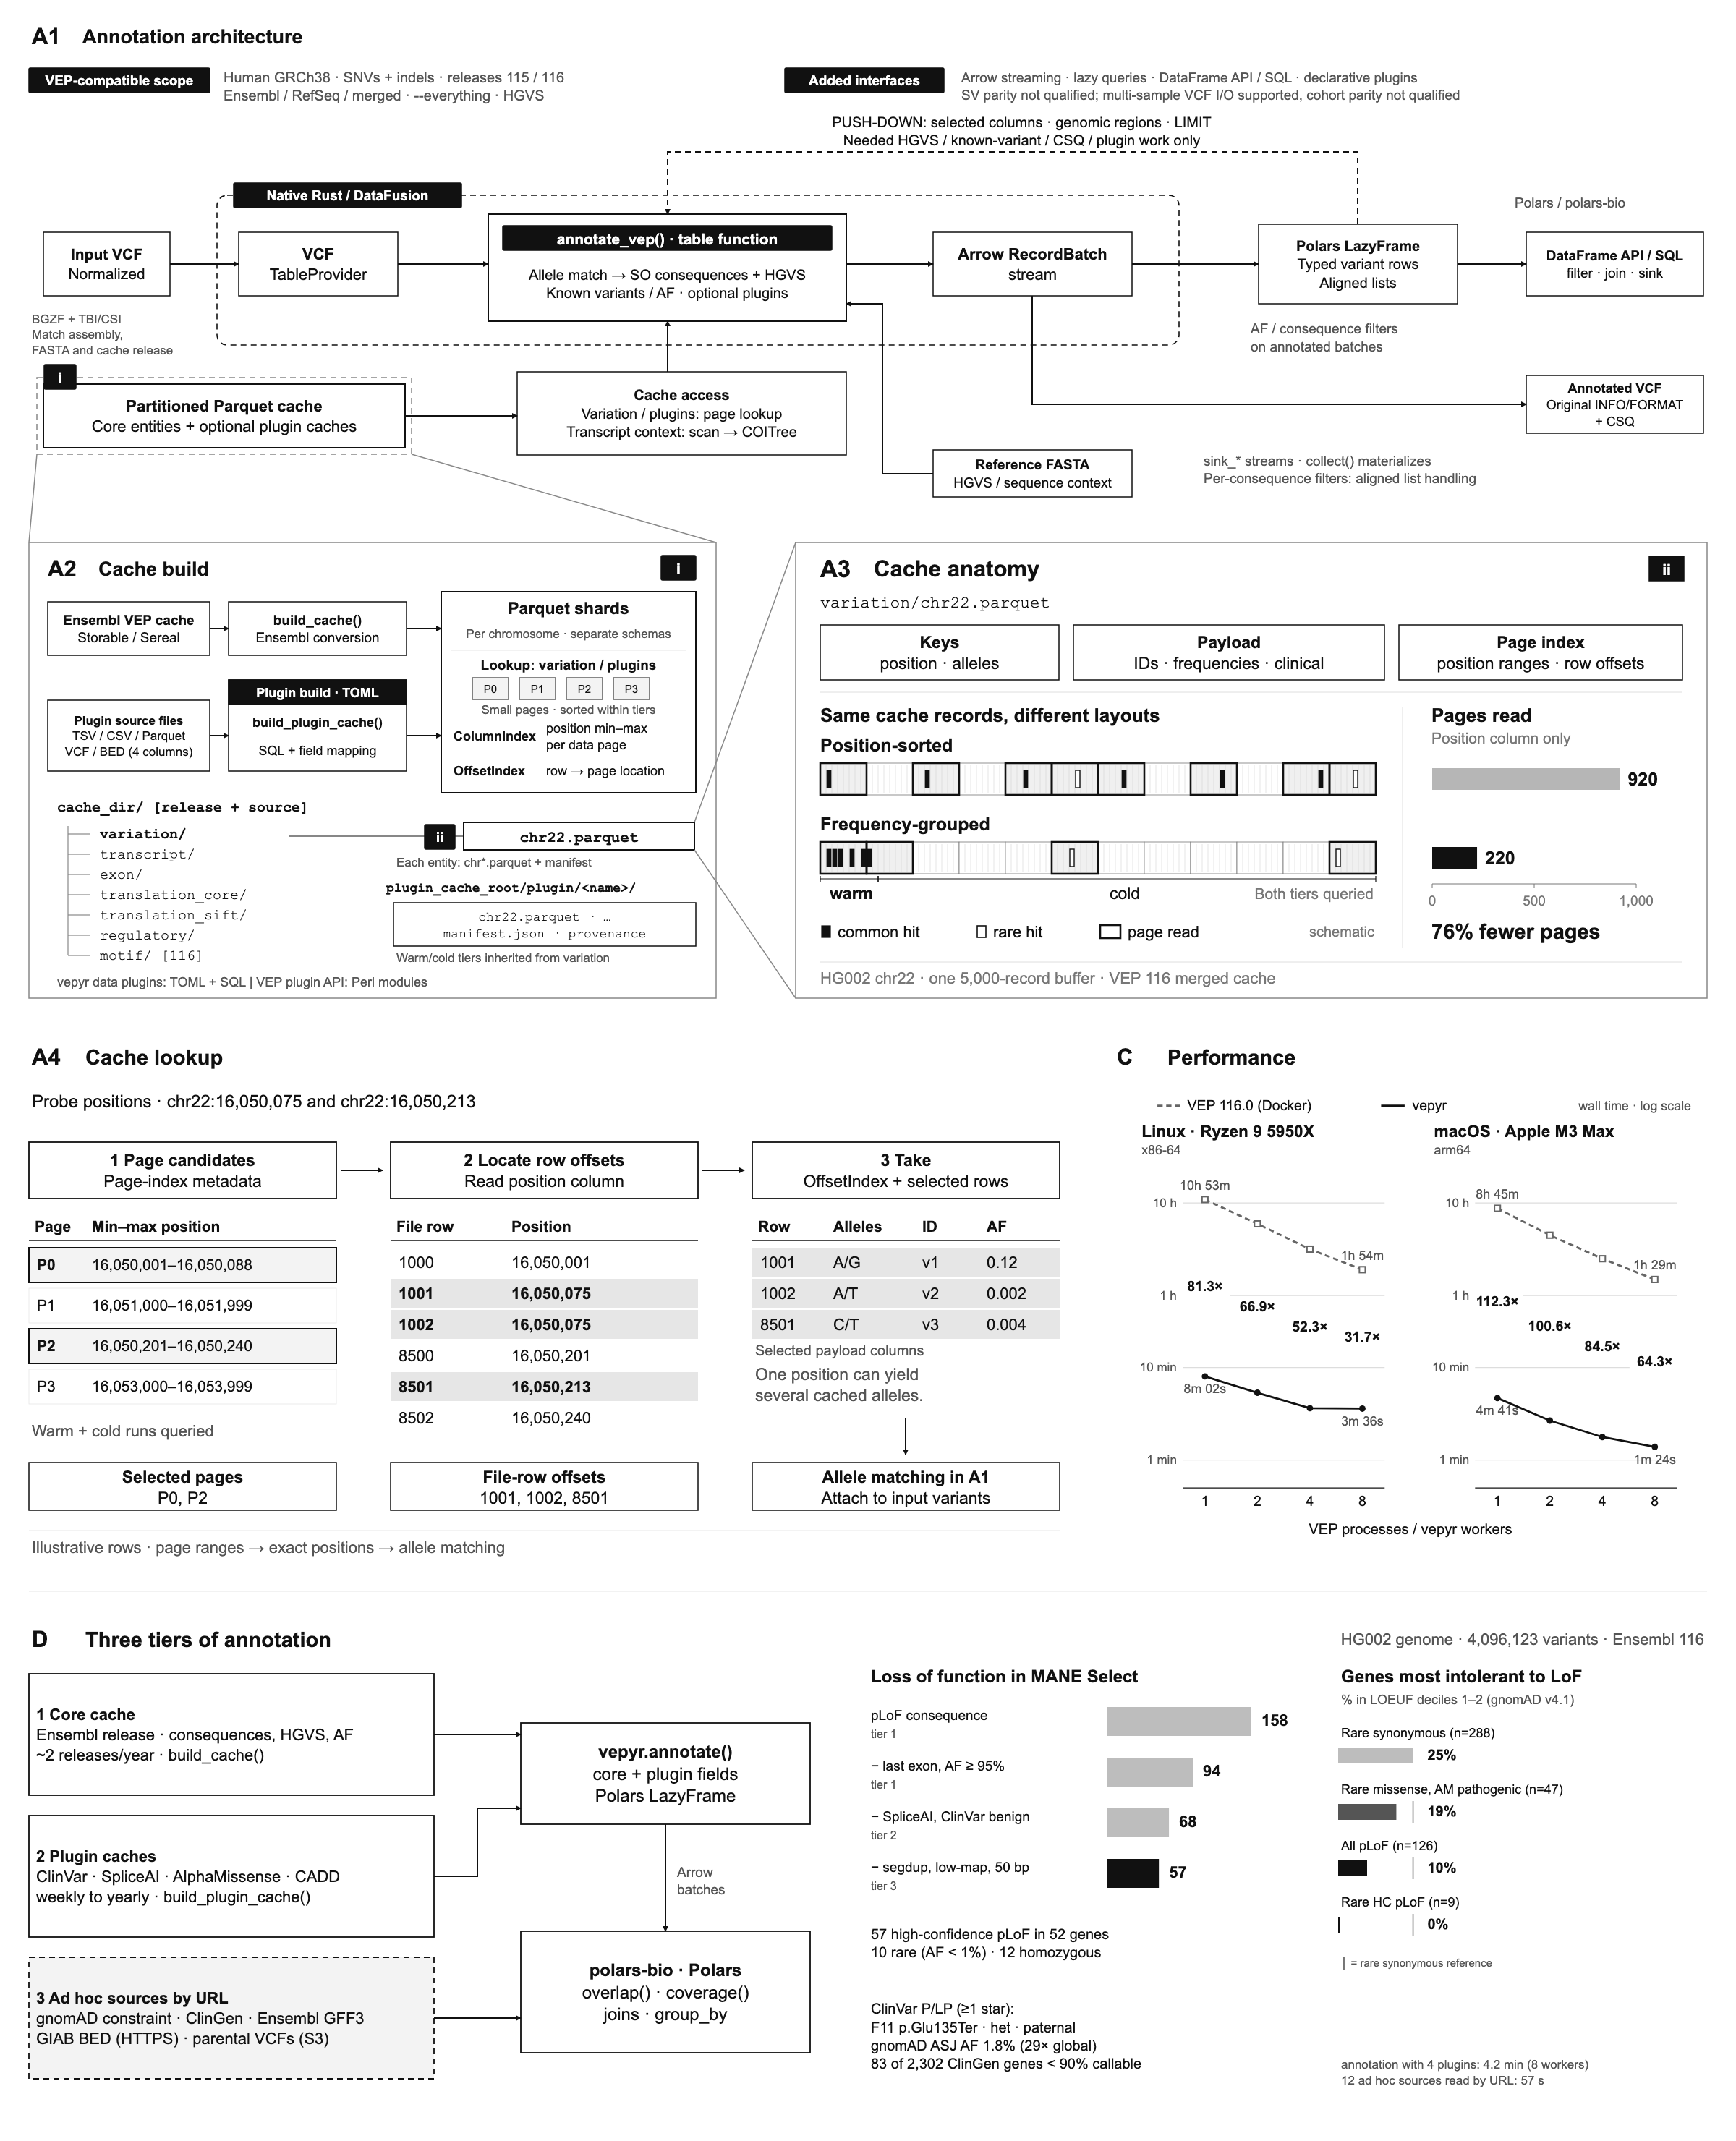
\includegraphics[width=\textwidth]{../figure1/figure1-tiered-annotation-proposal.png}
\caption*{Figure~1 (cache-workflow proposal) with the new panel~D in place of
the previous one, for checking proportions. Panels A1--A4 and C are
unchanged.}
\end{figure}
